\documentclass{beamer}

\usetheme{Madrid}
\usepackage{listings}
\usepackage{xcolor}

\title{1.1.63}
\author{ee25btech11063 - Vejith}
\date{\today}

\lstset{
    basicstyle=\ttfamily\small,
    breaklines=true,
    frame=single
}

\begin{document}

%---------------------------------
\begin{frame}
\titlepage
\end{frame}

%---------------------------------
\begin{frame}{Question}
The natural frequency of the system shown below is \hspace{1cm}(ME 2007)
\begin{figure}[H]
    \centering
    
\includegraphics[width=0.8\columnwidth]{figs/01.png}
    \label{fig:placeholder}
\end{figure}
\begin{enumerate}[label=\alph*)]
\begin{multicols}
     \item $\sqrt{\frac{k}{2m}}$
      \item $\sqrt{\frac{k}{m}}$
      \item $\sqrt{\frac{2k}{m}}$
      \item $\sqrt{\frac{3k}{m}}$
\end{multicols}
   \end{enumerate}
\end{frame}
\begin{frame}{Solution}
    Two springs of stiffness $k/2$ are connected in parallel, and this combination is in series with a spring of stiffness $k$, attached to a mass $m$. \bigskip

\textbf{Parallel Combination :} \\ 
Springs are in parallel when they have the same displacement. The equivalent stiffness is:
\begin{align}
    k_{\text{parallel}} = k_1 + k_2
\end{align}


Here,
\begin{align}
    k_{\text{parallel}} = \frac{k}{2} + \frac{k}{2} = k 
\end{align}


\end{frame}
\begin{frame}{Solution}
\textbf{Series Combination :} \\
   Springs are in series when they experience the same force. The equivalent stiffness is:
\begin{align}
    \frac{1}{k_{\text{eq}}} = \frac{1}{k_1} + \frac{1}{k_2}
\end{align}


Thus,
\begin{align}
    \frac{1}{k_{\text{eq}}} = \frac{1}{k} + \frac{1}{k} = \frac{2}{k}
\end{align}

\begin{align}
    k_{\text{eq}} = \frac{k}{2}
\end{align}


\bigskip
\end{frame}
\begin{frame}{Conclusion}
    \textbf{Natural Frequency :}

The natural frequency is given by:
\begin{align}
    \omega_n = \sqrt{\frac{k_{\text{eq}}}{m}}
\end{align}


Substituting,
\begin{align}
  \implies  \omega_n = \sqrt{\frac{k}{2m}}
\end{align}


\end{frame}
\begin{frame}{Python plot}
    \begin{figure}
        \centering
        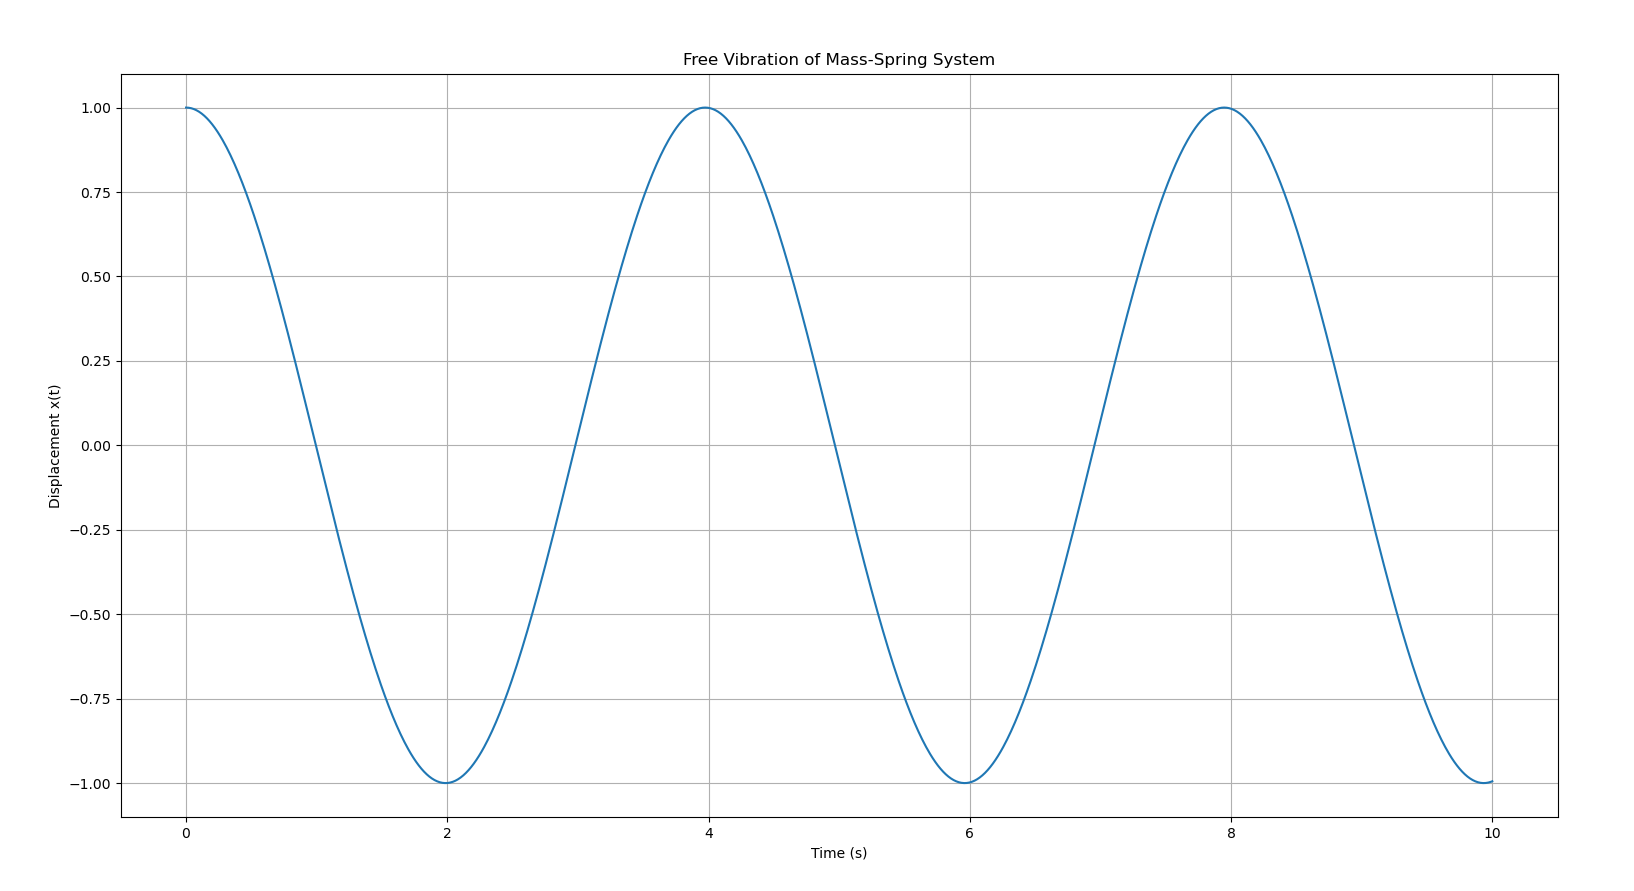
\includegraphics[width=1.0\linewidth]{figs/02.png}
        \label{fig:placeholder}
    \end{figure}
\end{frame}
\begin{frame}[fragile]{Python: plot.py}
\begin{lstlisting}[language=Python]
import numpy as np
import matplotlib.pyplot as plt
k = 10        
m = 2         
A = 1         
k_eq = k / 2
omega_n = np.sqrt(k_eq / m)
t = np.linspace(0, 10, 1000)
x = A * np.cos(omega_n * t)
plt.figure()
plt.plot(t, x)
plt.xlabel('Time (s)')
plt.ylabel('Displacement x(t)')
plt.title('Free Vibration of Mass-Spring System')
plt.grid()
plt.show()
\end{lstlisting}
\end{frame}
\end{document}
